The results of the estimation procedure is shown in Figure \ref{EX_pi0}.  Based on these values of $\pi_1$, $\mu_1$, $\sigma_1$, power predictions for different thresholding methods and a range of $n^*$'s are shown in Figure \ref{EX_power}.

\begin{center}
\begin{figure}[h]
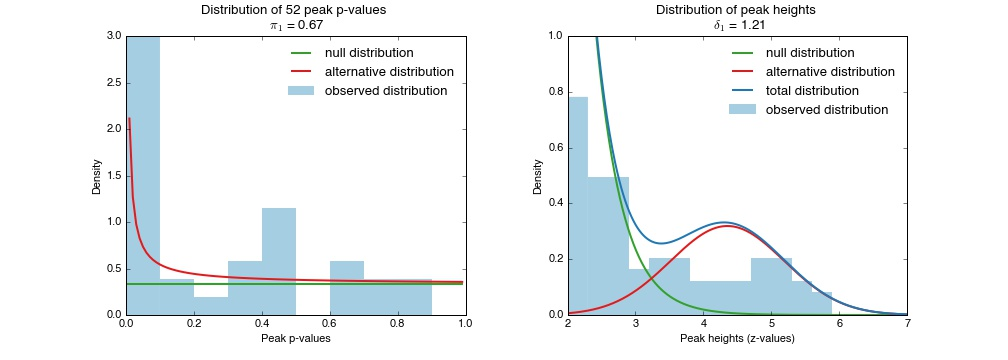
\includegraphics[scale=0.4]{FIG_EX_pi0.jpg}
\caption{Left: Estimated distribution of peak $p$-values.  The histogram of peak $p$-values is shown in light blue, the lines show the estimated part of the histogram stemming from the null distribution (green) and the total distribution (blue).  Right: Estimated distribution of peak heights.  The histogram of the peak heights is shown in light blue, the lines show the estimated distributions for the null (dark green), the alternative (light green) and the total distribution (blue) \label{EX_pi0}}
\end{figure}
\end{center}

%\textbf{TN: Now, if you're Ruth, you're probably not going to be happy that the retrospective power of her study (with her voxelwise RFT FWER) 39\%... but there it is.  ALSO, Ruth might say:  Well, average power wasn't important to me, what was important was Familywise power, detecting *anything*.  Is it easy to cook up those results?  It might actually make a nice accompaniment to these average power results.}

The results of the power estimation procedure can be found in Figure \ref{EX_power}. If the aim of the power analysis is to obtain at least 80\% average power, then this study would require 15 subjects for uncorrected thresholding at $\alpha=0.05$.  False discovery rate thresholding at $\alpha=0.05$ requires 16 subjects.  For family-wise error rate control at $\alpha=0.05$, the study would require 47 subjects with Random Field Theory thresholding.

%If one aims for familywise power - finding at least one true effect - then the current analysis does not require more subjects.  Using this model, we estimate that at least one true effect is found.

%\todo[inline]{Tom: You need to channel your inner John Ioannids!!  What does he say about the value of retrospective power?! To gague the belivability of the results!!! Joke: I have removed the part on retrospective power and focused on 80\% power.  Do I still need to say something about retrospective power? }


%It can be seen that in the current study, uncorrected testing at $\alpha=0.05$ leads to a power of 64\%, with $\alpha=0.001$ the power drops to 8\%.  RFT thresholding results in a power of 39\%.  A false discovery rate control with the method of \citep{Storey2001}, further denoted as $Q$, results in a power of 51\%.  False discovery rate control with the method of \citet{Benjamini1995}, like RFT control, results in a power of 39\%  Lastly, the power with familywise error rate control at 0.05 is the lowest, and equals $6\%$.

%The results indicate that thresholding with adaptive FDR control leads to more powerful results than uncorrected false positive rate control at the same $\alpha$-level of 5\%.  While this finding might seem contradictory, it has already been described by \citet{Reiss2012} and only occurs when the number of selected tests exceeds the number of positive tests (i.e. the number of selected peaks is higher than number of active peaks), which is likely to happen when $\pi_0$ is relatively small.


\begin{figure}
\begin{center}
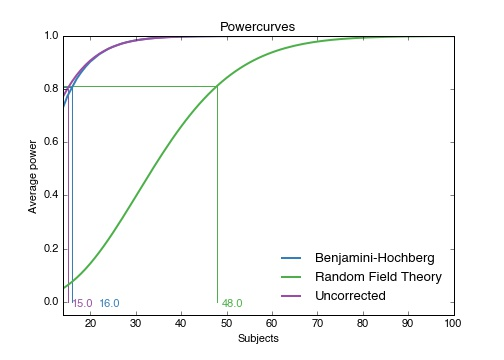
\includegraphics[scale=0.55]{FIG_EX_power.jpg}
\caption{Estimated peakwise average power, $u=2.5$ for different multiple testing procedures as a function of sample size.  The vertical lines show for each multiple testing procedure the required number of subjects to obtain a power of at least 80\%. \label{EX_power}}
\end{center}
\end{figure}

%\textbf{TN: There's something odd here that is worth mentioning either here or in the text... In the HCP evaluations (Figure 5), FDR-Q always had worse power than FDR-BH.  As $pFDR>=FDR$, this makes sense (if the 5\% FDR is $t$, then $pFDR>5\%$, and a more stringent $t'>t$ is needed that will necessarily be less powerful). HOWEVER, for this one dataset here, we find FDRQ more poweful than BH FDR... any idea about how this is?  I assume this is just a quirk of the Q=13 subjects dataset, AND/OR a reflection of the fact that FDR-Q incorprates an adaptive estimate of the null proportion, giving a less conservative inference, while BH FDR is conservative by a factor of $1/(1-pi1)$ right?}
